\section{Theory}

\subsection*{Binary Addition}
Addition of binary numbers follow the same logical rules as that of decimal numbers. 1 bit addition rules are shown below. To accomodate the carry bit, we use two bits of output.

\[
\begin{array}{@{}cr@{\,\,\,\,\,\,}rr@{\,\,\,\,\,\,}rr@{\,\,\,\,\,\,}rr}
    & 0 & & 0 & & 1 & & 1\\
+  & 0 & + & 1& + & 0& + & 1\\ \hline
  & 00 & & 01 && 01 && 11
\end{array}
\]

\subsubsection*{Half Adder Circuit}

The logic table for the 1 bit addition can be formed as follows, (where C represents the carry bit)

\begin{table}[H]
    \centering
    \begin{tabular}{|c|c|c|c|}\hline
    A & B & Q & C \\ \hline
    0 & 0 & 0 & 0 \\ 
    0 & 1 & 1 & 0 \\ 
    1 & 0 & 1 & 0 \\ 
    1 & 1 & 0 & 1 \\ \hline
    \end{tabular}
    \caption{1-bit Adder with Carry-Out}
\end{table}

One can observe that we can implement sum Q using an \verb|XOR| gate and carry bit C using an \verb|AND| gate.

\begin{figure}[H]
    \centering
    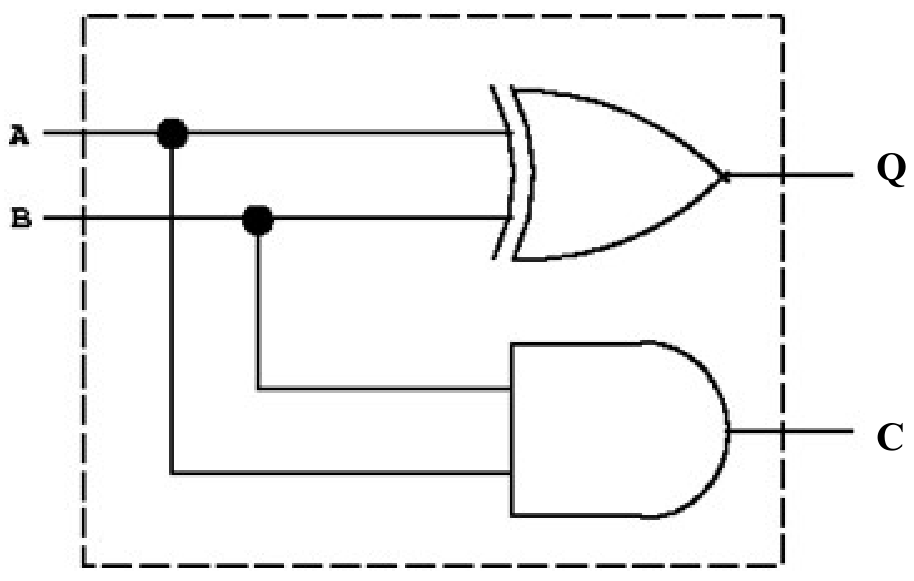
\includegraphics[width=0.5\columnwidth]{images/half-adder.png}
    \caption{Schematic for the half adder circuit}
    \label{half-adder}
\end{figure}

\subsubsection*{Full Adder Circuit}

To add two or more bits together we need to account for the carry-in bit from the previous operation. A full adder circuit accepts a carry in bit C$_{N-1}$ along with inputs A and B. The truth table will be formed as follows.

\begin{table}[H]
    \centering
    \begin{tabular}{|c|c|c|c|c|}\hline
    C$_{N-1}$ & A & B & Q & C$_N$ \\ \hline
    0 & 0 & 0 & 0 & 0 \\ 
    0 & 0 & 1 & 1 & 0 \\ 
    0 & 1 & 0 & 1 & 0 \\ 
    0 & 1 & 1 & 0 & 1 \\
    1 & 0 & 0 & 1 & 0 \\ 
    1 & 0 & 1 & 0 & 1 \\ 
    1 & 1 & 0 & 0 & 1 \\ 
    1 & 1 & 1 & 1 & 1 \\ \hline
    \end{tabular}
    \caption{One-bit Full Adder with Carry-In \& Carry-Out}
\end{table}

We can observe that we can implement sum Q using an \verb|XOR| of the 3 inputs (an odd number of 1s results in a 1). Hence the full adder can be constructed from two half adders and an \verb|OR| gate.

\begin{figure}[H]
    \centering
    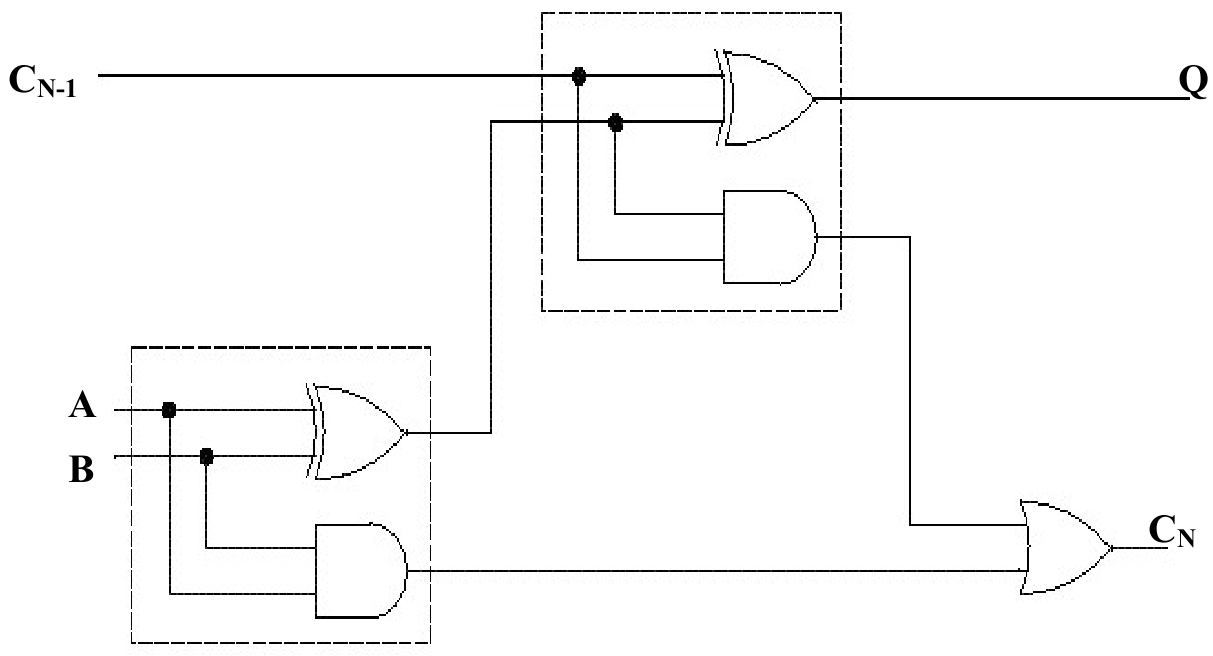
\includegraphics[width=0.85\columnwidth]{images/full-adder.png}
    \caption{Schematic for the full adder circuit}
    \label{full-adder}
\end{figure}

Now, to construct a 2-bit adder, we can combine a full adder with a half adder. Any arbitrary N-bit adder can thus be constructed by a cascading series of full adders, also called a \textit{ripple carry adder} (since the carry bit ripples from one stage to the next).

\begin{figure}[H]
    \centering
    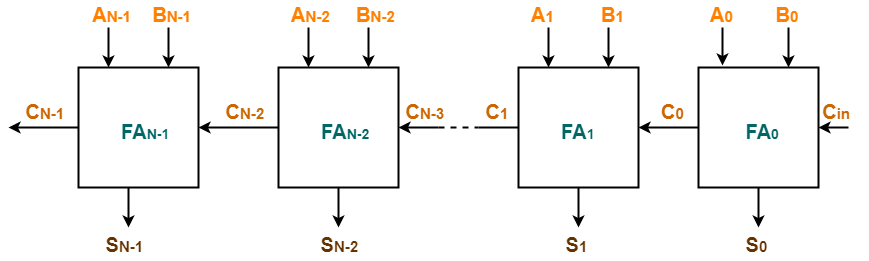
\includegraphics[width=0.9\columnwidth]{images/n-bit.png}
    \caption{Schematic for an N-bit ripple carry adder}
\end{figure}

However in a real circuit, gates take time to switch states, so 32-bit or 64-bit ripple carry adders might take a significant amount of time ($\sim$100 ns) to settle into their final sum. For this other adder circuits are used, like the \textit{carry look-ahead adder} which solves the delay by calculating the carry signals in advance.

% ========================================================================

\subsection*{Binary Subtraction}
Subtraction of binary numbers can be performed in a similar fashion. 1 bit subtraction rules are shown below. Here, to accomodate the borrow, we use two bits of output.

\[
\begin{array}{@{}cr@{\,\,\,\,\,\,}rr@{\,\,\,\,\,\,}rr@{\,\,\,\,\,\,}rr}
    & 0 & & 0 & & 1 & & 1\\
-  & 0 & - & 1& - & 0& - & 1\\ \hline
  & 00 & & 11 && 01 && 00
\end{array}
\]

\subsubsection*{Half Subtractor Circuit}

The logic table for the 1 bit subtraction is shown below (where B$_N$ represents the borrow bit)

\begin{table}[H]
    \centering
    \begin{tabular}{|c|c|c|c|}\hline
    A & B & Q & B$_N$ \\ \hline
    0 & 0 & 0 & 0 \\ 
    0 & 1 & 1 & 1 \\ 
    1 & 0 & 1 & 0 \\ 
    1 & 1 & 0 & 0 \\ \hline
    \end{tabular}
    \caption{1-bit subtractor with borrow}
\end{table}

One can observe that we can implement sum Q using an \verb|XOR| gate and borrow bit B$_N$ using an \verb|AND| gate with input A inverted.

\begin{figure}[H]
    \centering
    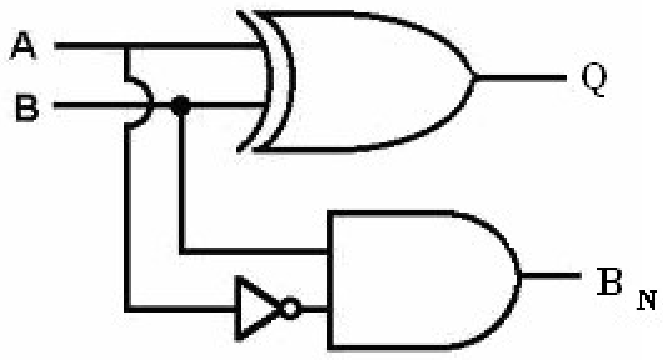
\includegraphics[width=0.4\columnwidth]{images/half-sub.png}
    \caption{Schematic for the half subtractor circuit}
    \label{half-sub}
\end{figure}

\subsubsection*{Full Subtractor Circuit}

A full subtractor circuit accepts a minuend (A) and the subtrahend (B) and a borrow (B$_{N-1}$) as inputs from a previous circuit.

\begin{table}[H]
    \centering
    \begin{tabular}{|c|c|c|c|c|}\hline
    B$_{N-1}$ & A & B & Q & B$_N$ \\ \hline
    0 & 0 & 0 & 0 & 0 \\ 
    0 & 0 & 1 & 1 & 1 \\ 
    0 & 1 & 0 & 1 & 0 \\ 
    0 & 1 & 1 & 0 & 0 \\
    1 & 0 & 0 & 1 & 1 \\ 
    1 & 0 & 1 & 0 & 1 \\ 
    1 & 1 & 0 & 0 & 0 \\ 
    1 & 1 & 1 & 1 & 1 \\ \hline
    \end{tabular}
    \caption{1-bit Full Subtractor with B$_{N-1}$ \& B$_N$}
\end{table}

A full subtractor circuit can be constructed by combining two half subtractor circuits and an \verb|OR| gate.

\begin{figure}[H]
    \centering
    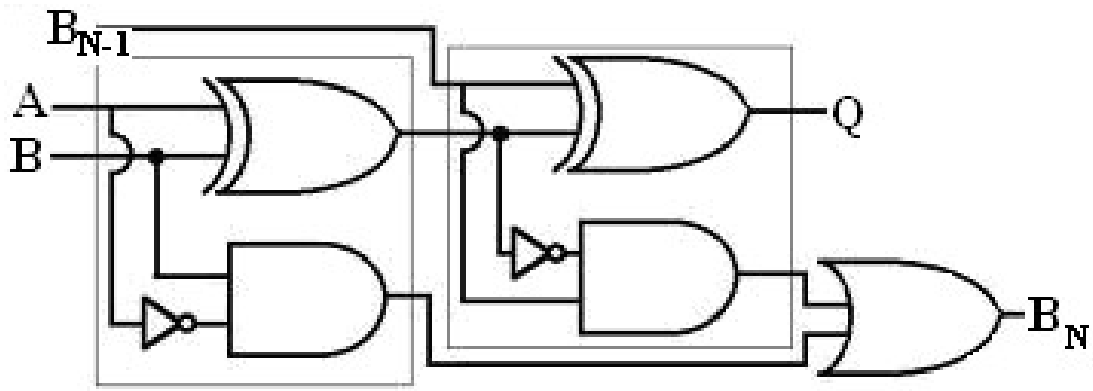
\includegraphics[width=0.7\columnwidth]{images/full-sub.png}
    \caption{Schematic for the full subtractor circuit}
    \label{full-sub}
\end{figure}

\subsection*{Full Adder Subtractor Circuit}
To use the same circuit to perform both addition and subtraction, one can replace the \verb|NOT| gate of the subtractor circuit by an \verb|XOR| gate. Here, the second input for the \verb|XOR| gate decides the function of the circuit, either addition or subtraction. If the second input for \verb|XOR| is 0, the circuit will do addition and if 1, it will do subtraction. Hence they act as a \textit{control bits} ($X_1$ and $X_2$).

\begin{figure}[H]
    \centering
    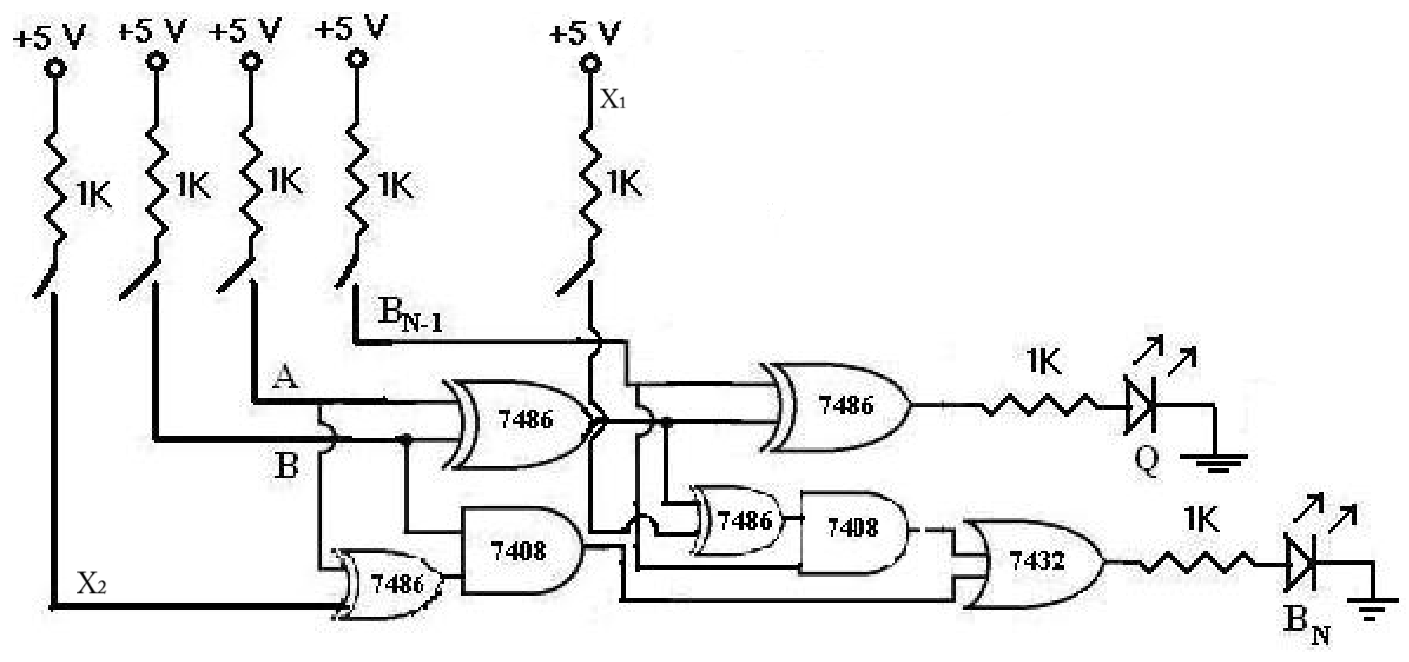
\includegraphics[width=1\columnwidth]{images/full-comb.png}
    \caption{Full Adder-Subtractor Circuit Diagram}
    \label{full-add-sub}
\end{figure}

N-bit subtractor circuits can also be built using ripple borrow subtractor technique, similar to the one described before.
% ======================================================================================
\section{Experimental Setup}
\subsection*{Apparatus}

\begin{enumerate}
    \item Digital ICs (XOR-7486, AND-7408, OR-7432, NOT-7404) 
    \item Resistors (1 k$\Omega$)
    \item D.C. Power supply (5V)
    \item LEDs
    \item Connecting Wires
    \item Multimeters
\end{enumerate}

\subsection*{Circuit Diagrams}
\begin{figure}[H]
    \centering
    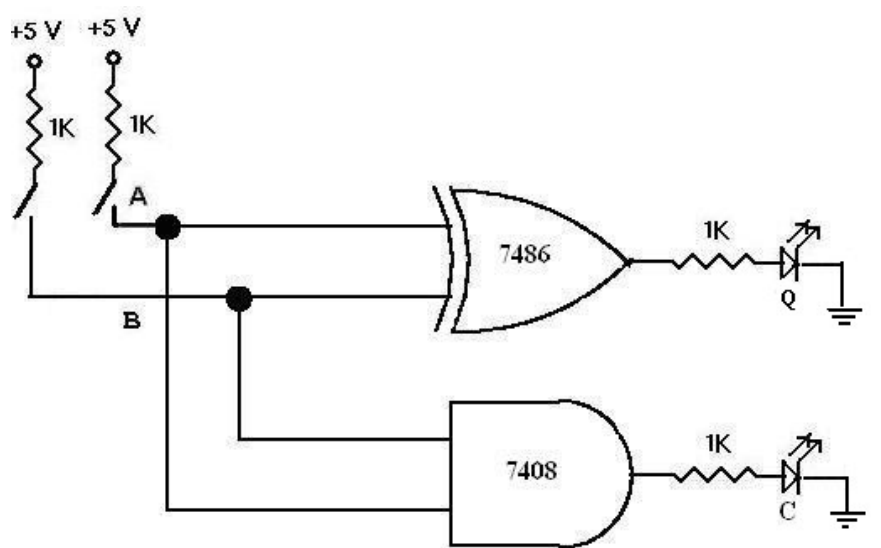
\includegraphics[width=0.55\columnwidth]{images/c-half-add.png}
    \caption{Half Adder Circuit Diagram}
    \label{half-add}
\end{figure}

\begin{figure}[H]
    \centering
    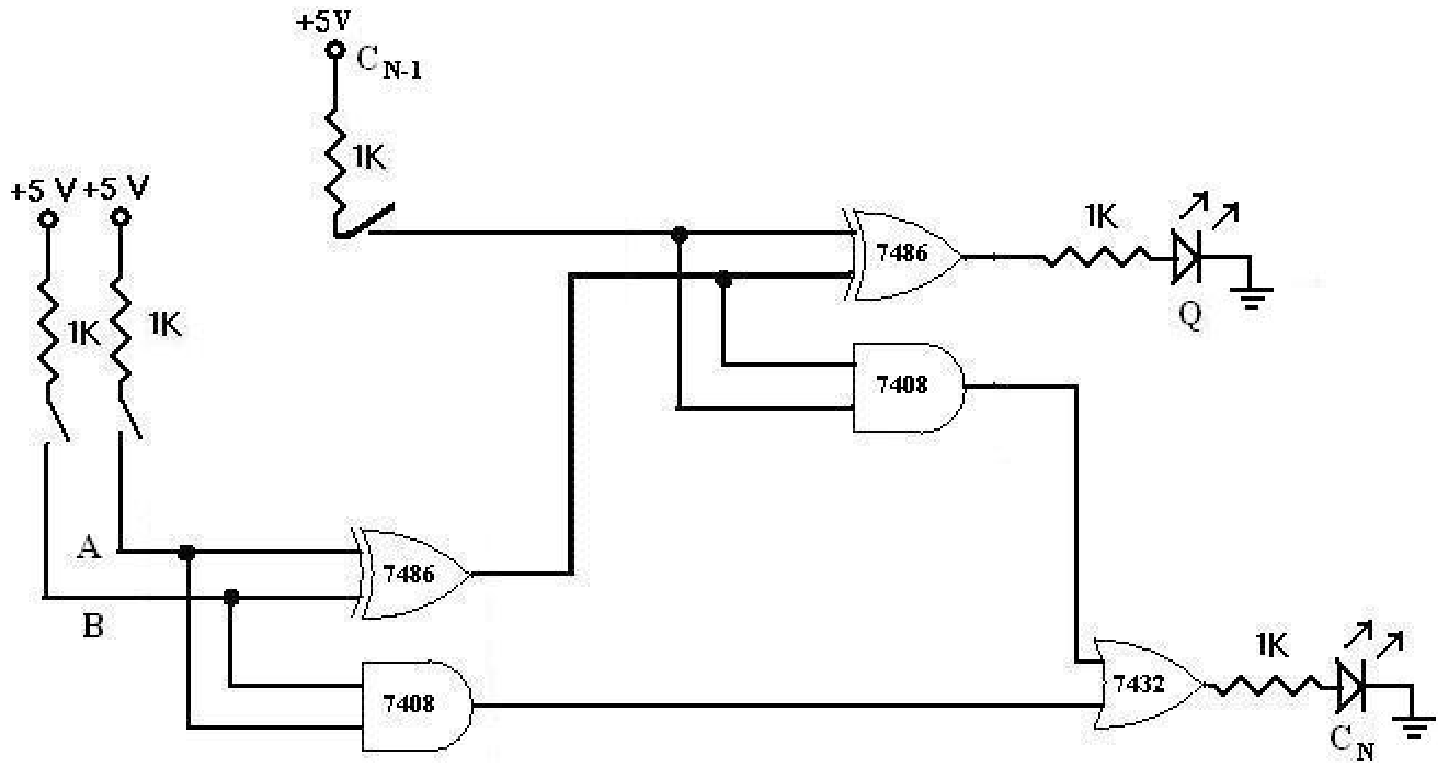
\includegraphics[width=0.8\columnwidth]{images/c-full-add.png}
    \caption{Full Adder Circuit Diagram}
    \label{full-add}
\end{figure}

\begin{figure}[H]
    \centering
    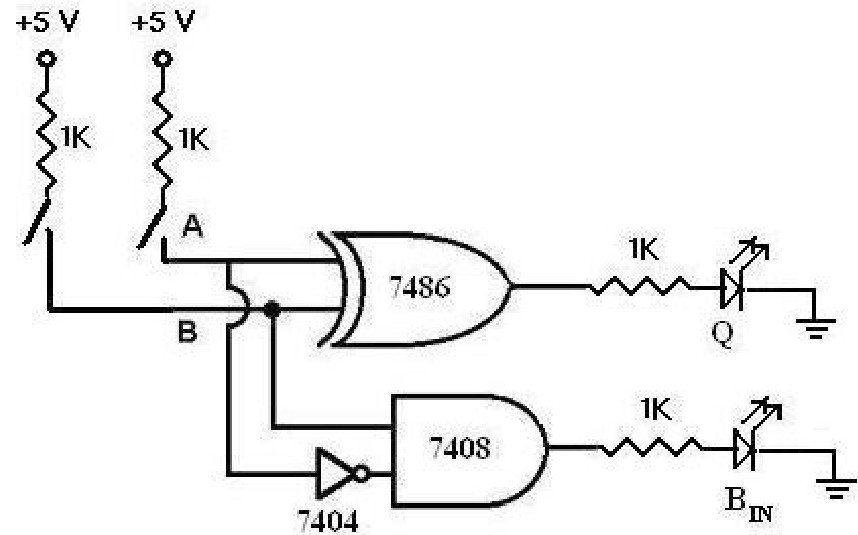
\includegraphics[width=0.5\columnwidth]{images/c-half-sub.png}
    \caption{Half Subtractor Circuit Diagram}
    \label{half-subt}
\end{figure}

\begin{figure}[H]
    \centering
    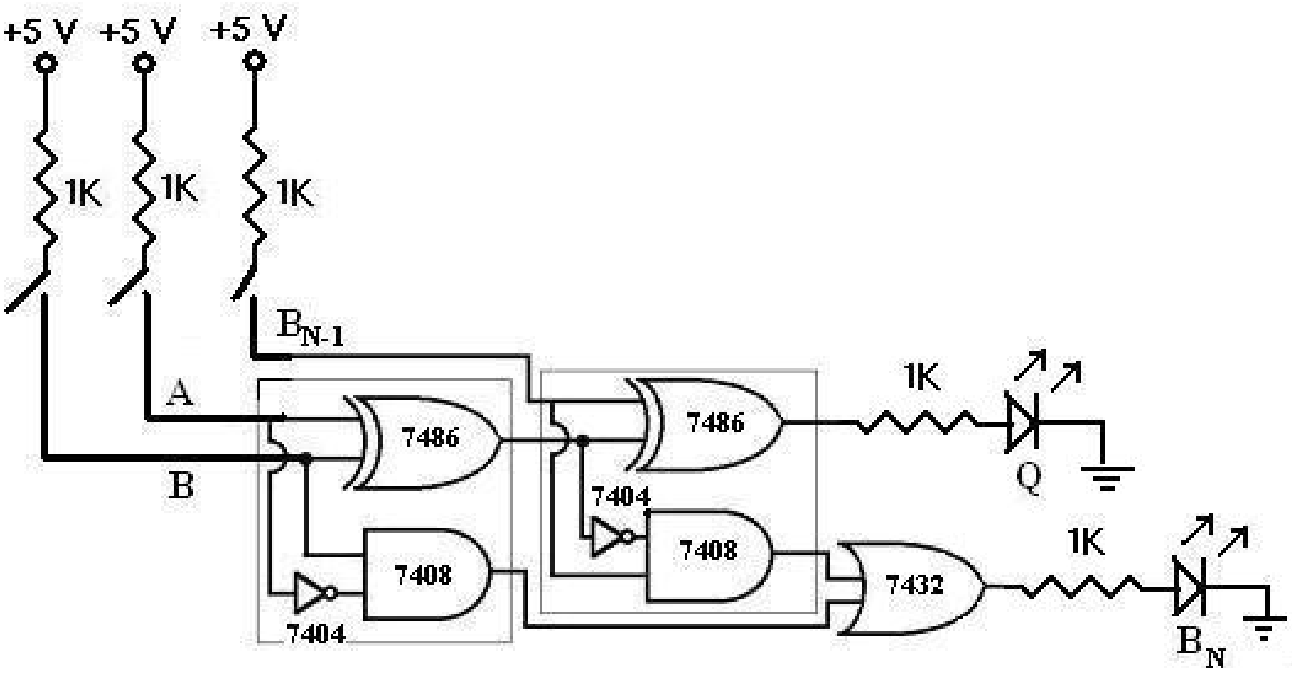
\includegraphics[width=0.85\columnwidth]{images/c-full-sub.png}
    \caption{Full Subtractor Circuit Diagram}
    \label{full-subt}
\end{figure}

\subsection*{Pinout Diagrams}
\begin{figure}[H]
    \centering
    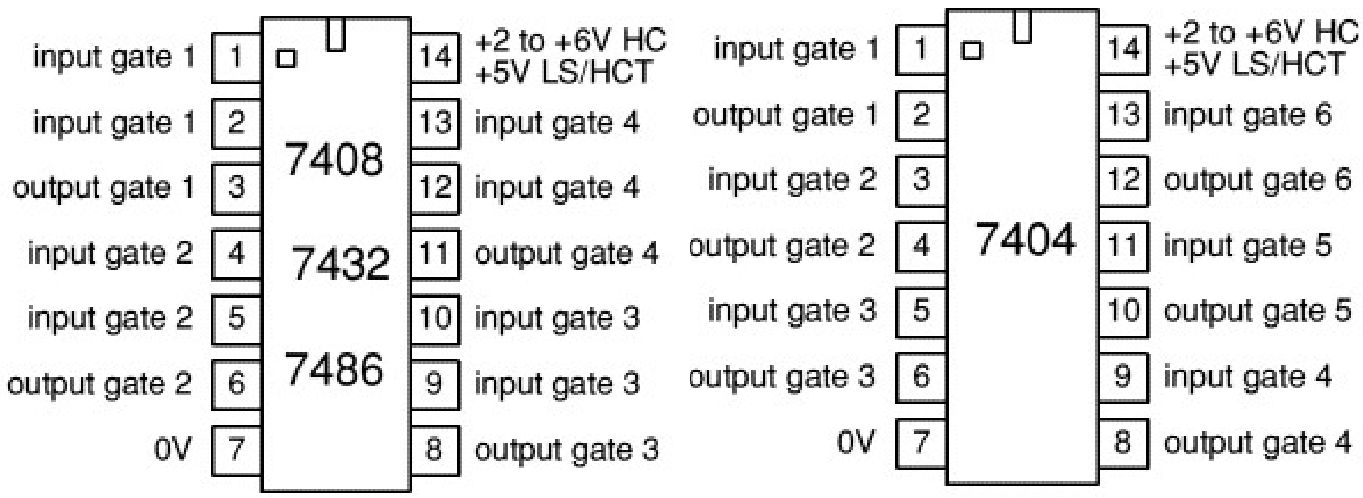
\includegraphics[width=1\columnwidth]{images/pinout.png}
    \caption{Pin connections for different ICs used in this experiment}
    \label{pinout}
\end{figure}